\documentclass[12pt]{article}
\usepackage{mathtools}
\usepackage[papersize={210mm, 270mm},tmargin=17mm,bmargin=15mm,lmargin=15mm,rmargin=15mm]{geometry}
\usepackage[utf8]{inputenc}
\usepackage{graphicx}
\usepackage{fancyhdr}
\usepackage{tikz}
\usepackage{whilecode2}
\usepackage{listings}
\usetikzlibrary{positioning}
\usetikzlibrary{arrows.meta, automata, positioning, quotes}
\pagestyle{fancy}
\lhead[\thepage]{David Cuesta Martín}
\rhead[David Cuesta Martín]{\thepage}
\cfoot{}
\author{David }


\begin{document}
\section*{Ejercicio 1: }
Codificar el programa con la codificación más pequeña que diverge:\\
En primer lugar, averiguamos cual es el más simple, el cual es:\\

\whileprogram{Q}{0}{
}{s}
\begin{whilecode}[H]

$X_2 \Assig X_1 + 1$\;
             \While{$X_2 \not = 0$}{
              $X_1 \Assig 0$
             }
\end{whilecode} 

Por tanto ahora realizamos $while2N(Q)$: \\

$while2N((0,\ X_2:=X_1+1;\ while\ X_2\neq 0\ do\ X_1:=0\ od))= \sigma_1^2(0,code2N(s))=\\ \sigma_1^2(0,\Gamma(sent2N(X_2:=X_1+1), sent2N(while\ X_2 \not =\ 0\ do\ X_1:=0\ od))-1)=\\ 
\sigma_1^2(0,\Gamma(5\sigma^2_1(1,0)+2, 5\sigma^2_1(1, code2N(X_1:=0))+4)-1)=\\ 
\sigma_1^2(0,\Gamma(7, 5\sigma^2_1(1, \Gamma(0)-1)+4)-1)=\\ 
\sigma_1^2(0,\Gamma(7, 5\sigma^2_1(1, \sigma_1^2(0,0))+4)-1)=\\ 
\sigma_1^2(0,\Gamma(7, 5\sigma^2_1(1, \sigma_1^2(0,0))+4)-1)=\\
\sigma_1^2(0,\Gamma(7, 9)-1)=
\sigma_1^2(0,\sigma_1^2(1,\sigma_1^2(7,9)))=
\sigma_1^2(0,\sigma_1^2(1,145))=
\sigma_1^2(0,10876)= \boxed{59160002}$

\section*{Ejercicio 2:}
Hacer programa en Octave que genere todos los vectores:\\
El código, con ayuda de los programas proporcionados, es facil de deducir:\\ \\
\begin{verbatim}
    function vectores ()
i=0;
while (0<=0)
disp(['(' num2str(godeldecoding(i)) ')' ]);
i=i+1;
end

end
\end{verbatim}
Este programa nos imprime en pantalla todos los vectores, es decir, al haber infinitos vectores, el programa nunca para de ejecutarse.
Ejemplo de ejecución:
\begin{center}
    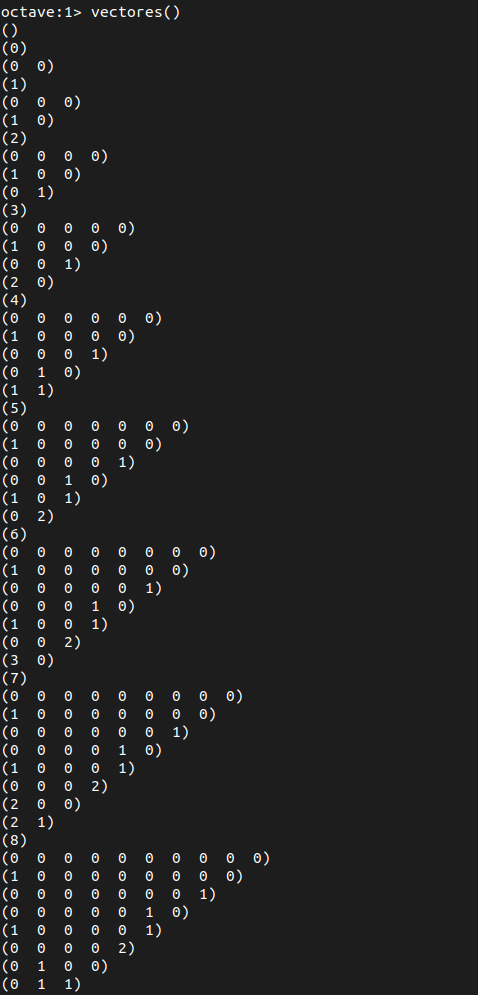
\includegraphics[width=10cm]{vectors.png}
\end{center}
\newpage
\section*{Ejercicio 3:}
Hacer programa en Octave que genere todos los programas while:
También es facil de deducir:
\begin{verbatim}
    function vectores ()
i=0;
while (0<=0)
disp([N2WHILE(i)]);
i=i+1;
end

end
\end{verbatim}
\\ Y el ejemplo de ejecución es:
\begin{center}
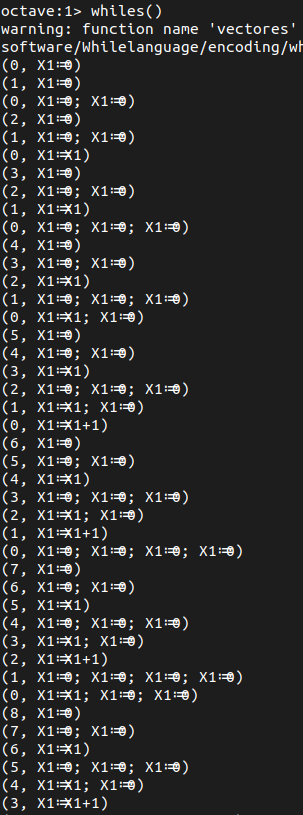
\includegraphics[width=6cm]{whiles.png}
\end{center}


\end{document}
